\documentclass[12pt]{report}
\usepackage[utf8]{inputenc}
\usepackage[russian]{babel}
%\usepackage[14pt]{extsizes}
\usepackage{listings}
\usepackage{graphicx}
\usepackage{amsmath,amsfonts,amssymb,amsthm,mathtools} 
\usepackage{pgfplots}
\usepackage{filecontents}
\usepackage{float}
\usepackage{comment}
\usepackage{indentfirst}
\usepackage{eucal}
\usepackage{enumitem}
%s\documentclass[openany]{book}
\frenchspacing

\usepackage{indentfirst} % Красная строка

\usetikzlibrary{datavisualization}
\usetikzlibrary{datavisualization.formats.functions}

\usepackage{amsmath}


% Для листинга кода:
\lstset{ %
	language=c,                 % выбор языка для подсветки (здесь это С)
	basicstyle=\small\sffamily, % размер и начертание шрифта для подсветки кода
	numbers=left,               % где поставить нумерацию строк (слева\справа)
	numberstyle=\tiny,           % размер шрифта для номеров строк
	stepnumber=1,                   % размер шага между двумя номерами строк
	numbersep=5pt,                % как далеко отстоят номера строк от подсвечиваемого кода
	showspaces=false,            % показывать или нет пробелы специальными отступами
	showstringspaces=false,      % показывать или нет пробелы в строках
	showtabs=false,             % показывать или нет табуляцию в строках
	frame=single,              % рисовать рамку вокруг кода
	tabsize=2,                 % размер табуляции по умолчанию равен 2 пробелам
	captionpos=t,              % позиция заголовка вверху [t] или внизу [b] 
	breaklines=true,           % автоматически переносить строки (да\нет)
	breakatwhitespace=false, % переносить строки только если есть пробел
	escapeinside={\#*}{*)}   % если нужно добавить комментарии в коде
}


\usepackage[left=2cm,right=2cm, top=2cm,bottom=2cm,bindingoffset=0cm]{geometry}
% Для измененных титулов глав:
\usepackage{titlesec, blindtext, color} % подключаем нужные пакеты
\definecolor{gray75}{gray}{0.75} % определяем цвет
\newcommand{\hsp}{\hspace{20pt}} % длина линии в 20pt
% titleformat определяет стиль
\titleformat{\chapter}[hang]{\Huge\bfseries}{\thechapter\hsp\textcolor{gray75}{|}\hsp}{0pt}{\Huge\bfseries}


% plot
\usepackage{pgfplots}
\usepackage{filecontents}
\usetikzlibrary{datavisualization}
\usetikzlibrary{datavisualization.formats.functions}

\begin{document}
	%\def\chaptername{} % убирает "Глава"
	\thispagestyle{empty}
	\begin{titlepage}
		\noindent \begin{minipage}{0.15\textwidth}
			
\includegraphics[width=\linewidth]{img/b_logo}
		\end{minipage}
		\noindent\begin{minipage}{0.9\textwidth}\centering
			\textbf{Министерство науки и высшего образования Российской Федерации}\\
			\textbf{Федеральное государственное бюджетное образовательное учреждение высшего образования}\\
			\textbf{~~~«Московский государственный технический университет имени Н.Э.~Баумана}\\
			\textbf{(национальный исследовательский университет)»}\\
			\textbf{(МГТУ им. Н.Э.~Баумана)}
		\end{minipage}
		
		\noindent\rule{18cm}{3pt}
		\newline\newline
		\noindent ФАКУЛЬТЕТ $\underline{\text{«Информатика и системы управления»}}$ \newline\newline
		\noindent КАФЕДРА $\underline{\text{«Программное обеспечение ЭВМ и информационные технологии»}}$\newline\newline\newline\newline\newline
		
		\begin{center}
			\noindent\begin{minipage}{1.1\textwidth}\centering
				\Large\textbf{  Отчет по лабораторной работе №1}\newline
				\textbf{по дисциплине <<Математическая статистика>>}\newline\newline\newline
			\end{minipage}
		\end{center}
		
		\noindent\textbf{Тема} $\underline{\text{Гистрограмма и эмпирическая функция распределения}}$\newline\newline
		\noindent\textbf{Студент} $\underline{\text{Романов А.В.~~~~~~~~~~~~~~~~~~~~~~~~~~~~~~~~~~~~~~~~~~~~~~~~~~~~~}}$\newline\newline
		\noindent\textbf{Группа} $\underline{\text{ИУ7-63Б~~~~~~~~~~~~~~~~~~~~~~~~~~~~~~~~~~~~~~~~~~~~~~~~~~~~~~~~~~~~~}}$\newline\newlineg
		\noindent\textbf{Оценка (баллы)} $\underline{\text{~~~~~~~~~~~~~~~~~~~~~~~~~~~~~~~~~~~~~~~~~~~~~~~~~~~~~~~~~~~~}}$\newline\newline
		\noindent\textbf{Преподаватель} $\underline{\text{Саркисян П. С.~~~~~~~~~~~~~~~~~~~~~~~~~~~~~~~~~~~~~~~~~}}$\newline\newline\newline
		
		\begin{center}
			\vfill
			Москва~---~\the\year
			~г.
		\end{center}
	\end{titlepage}

\chapter*{Задание}

\section*{Цель работы}
Построение гистограммы и эмпирической функции распределения.

\section*{Постановка задачи}

\begin{enumerate}
	\item Для выборки объёма $n$ из генеральной совокупности $X$ реализовать в виде программы на ЭВМ
	\begin{enumerate}
		\item вычисление максимального значения $M_{\max}$ и минимального значения $M_{\min}$;
		\item размаха $R$ выборки;
		\item вычисление оценок $\hat\mu$ и $S^2$ математического ожидания $MX$ и дисперсии $DX$;
		\item группировку значений выборки в $m = [\log_2 n] + 2$ интервала;
		\item построение на одной координатной плоскости гистограммы и графика функции плотности распределения вероятностей нормальной случайной величины с математическим ожиданием $\hat{\mu}$ и дисперсией $S^2$;
		\item построение на другой координатной плоскости графика эмпирической функции распределения и функции распределения нормальной случайной величины с математическим ожиданием $\hat{\mu}$ и дисперсией $S^2$.
	\end{enumerate}
	\item Провести вычисления и построить графики для выборки из индивидуального варианта.
\end{enumerate}

\chapter*{Теоретические сведения}

\section*{Формулы для вычисления величин}

\subsection*{Минимальное и максимальное значения выборки}
\begin{equation}
	\begin{aligned}
	M_{\max} = X_{(n)}\\
	M_{\min} = X_{(1)}
	\end{aligned}
\end{equation}

\subsection*{Размах выборки}
\begin{equation}
	R = M_{\max} - M_{\min}.
\end{equation}

\subsection*{Оценки математического ожидания и дисперсии}
\begin{equation}
	\begin{aligned}
	\hat\mu(\vec X_n) &= \frac 1n \sum_{i=1}^n X_i\\
	S^2(\vec X_n) &= \frac 1{n-1} \sum_{i=1}^n (X_i-\overline X_n)^2
	\end{aligned}
\end{equation}

\section*{Определение эмпирической плотности и гистограммы}

Пусть $\vec x$ -- выборка из генеральной совокупности $X$. Если объем $n$ этой выборки велик, то значения $x_i$ группируют в интервальный статистический ряд. Для этого отрезок $J = [x_{(1)}, x_{(n)}]$ делят на $m$ равновеликих частей:

\begin{equation*}
	J_i = [x_{(1)} + (i - 1) \cdot \Delta, x_{(1)} + i \cdot \Delta), i = \overline{1; m - 1}
\end{equation*}

\begin{equation*}
	J_{m} = [x_{(1)} + (m - 1) \cdot \Delta, x_{(n)}]
\end{equation*}

\begin{equation*}
	\Delta = \frac{|J|}{m} = \frac{x_{(n)} - x_{(1)}}{m}
\end{equation*}

Интервальным статистическим рядом называют таблицу:

\begin{table}[htb]
	\centering
	\begin{tabular}{|c|c|c|c|c|}
		\hline
		$J_1$ & ... & $J_i$ & ... & $J_m$ \\
		\hline
		$n_1$ & ... & $n_i$ & ... & $n_m$ \\
		\hline
	\end{tabular}
\end{table}

где $n_i$ -- количество элементов выборки $\vec x$, которые $\in J_i$.

Обычно выборку разбивают на $m=[\log_2n]+2$ интервалов, где $n$ -- размер выборки.

Гистограмма -- это график эмпирической плотности. 

\textit{Эмпирической плотностью}, отвечающей выборке $\vec x$, называют функцию:
\begin{equation}
	\hat f(x) =
	\begin{cases}
	\frac{n_i}{n \Delta}, x \in J_i, i = \overline{1; m} \\
	0, \text{иначе} \\
	\end{cases}
\end{equation}

где $J_i$ -- полуинтервал статистического ряда, $n_i$ -- количество элементов выборки, входящих в полуинтервал, $n$ -- количество элементов выборки.

\section*{Определение эмпирической функции распределения}

Пусть $\vec x = (x_1, ..., x_n)$ -- выборка из генеральной совокупности $X$. Обозначим $n(x, \vec x)$ -- число элементов вектора $\vec x$, которые имеют значения меньше $x$.

\textit{Эмпирической функцией распределения} называют функцию $F_n: \mathbb{R} \to \mathbb{R}$, определенную как: 

\begin{equation}
	F_n(x) = \frac{n(x, \vec x)}{n}
\end{equation}

\chapter*{Результаты работы программы}

\section*{Код программы}

\begin{lstlisting}[language=Matlab]
X = [
	-10.82,-9.27,-9.65,-9.36,-9.27,-11.25,-9.89,-9.26,-11.15,-8.90,
	-11.02,-8.28,-9.18,-10.16,-10.59,-10.82,-9.05,-9.47,-10.98,-11.50,
	-8.64,-10.86,-10.76,-11.49,-11.09,-9.33,-9.32,-9.66,-8.79,-10.54,
	-9.12,-10.40,-8.59,-10.22,-9.06,-10.59,-10.60,-10.25,-9.35,-11.44,
	-9.81,-9.32,-9.95,-9.33,-10.64,-9.45,-10.99,-10.15,-10.39,-10.36,
	-10.49,-11.67,-10.00,-10.87,-11.11,-9.68,-10.77,-9.13,-8.62,-10.33,
	-11.36,-10.24,-9.41,-11.05,-10.15,-9.35,-11.45,-9.87,-10.41,-10.11,
	-10.84,-11.48,-7.77,-10.79,-9.88,-10.70,-9.07,-9.47,-10.15,-9.93,
	-11.52,-9.04,-10.93,-10.13,-9.56,-11.39,-9.79,-9.19,-11.09,-9.86,
	-10.67,-10.26,-9.07,-10.53,-11.24,-10.16,-11.33,-8.76,-8.88,-10.53,
	-10.12,-8.98,-9.84,-9.90,-10.13,-9.32,-9.31,-9.99,-8.55,-11.64,
	-11.32,-10.51,-11.71,-10.50,-10.50,-12.20,-11.68,-10.45,-7.88,-10.84
]

MAX_M = max(X);
MIN_M = min(X);

R = MAX_M - MIN_M;

MX = mean(X);
DX = var(X);

m = floor(log2(length(X))) + 2;
histo = histogram(X, m);

sigma_var = std(X);
x = (MIN_M - 1):(sigma_var / 100):(MAX_M + 1);
f = normpdf(x, MX, sigma_var);
figure;
heights = histo.Values / (sum(histo.Values) * histo.BinWidth);
c = [];

for k = 1:(length(histo.BinEdges) - 1)
	c = [c, (histo.BinEdges(k + 1) + histo.BinEdges(k)) / 2];
end

hold on;
bar(c, heights, 1); 
plot(x, f, 'r');

F = normcdf(x, MX, sigma_var); 
figure;
hold on;
ecdf(X); 
plot(x, F, 'g');
\end{lstlisting}

\section*{Результаты расчётов}

\begin{equation*}
M_{\min} = -12,2 \\
\end{equation*}
\begin{equation*}
M_{\max} = -7,77 \\
\end{equation*}
\begin{equation*}
R = 4,43 \\
\end{equation*}
\begin{equation*}
\hat\mu(\vec x_n) = -10,1318 \\
\end{equation*}
\begin{equation*}
S^2(\vec x_n) = 0,846 \\
\end{equation*}
\begin{equation*}
m = 8
\end{equation*}

\begin{figure}[H]
	\centering
	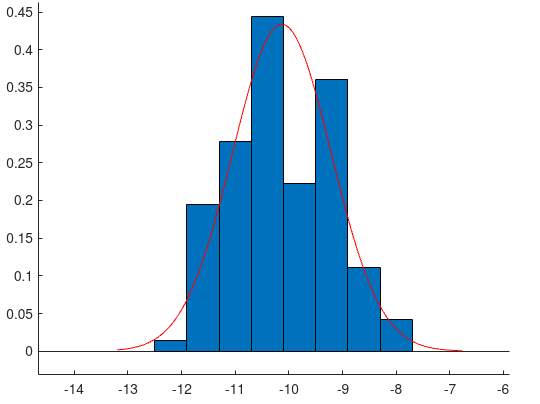
\includegraphics[scale=0.7]{img/1.png}
	\caption{Гистограмма и график функции плотности распределения вероятностей нормальной случайной величины с выборочными мат. ожиданием и дисперсией}
	\label{fig:1}
\end{figure}

\begin{figure}[H]
	\centering
	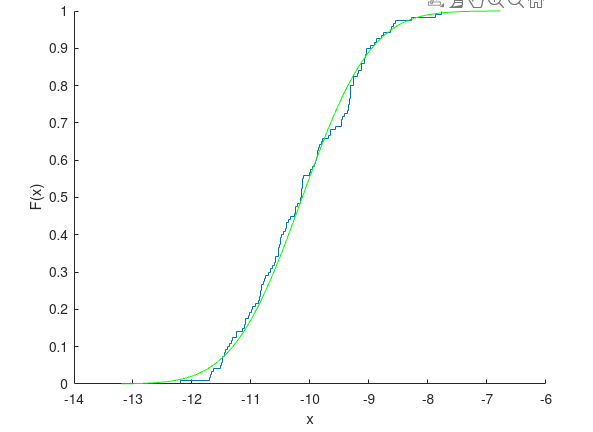
\includegraphics[scale=0.7]{img/2.png}
	\caption{График эмперической функции распределения и функции распределения нормальной случайной величины с выборочными мат. ожиданием и дисперсией}
	\label{fig:2}
\end{figure}

\bibliographystyle{utf8gost705u}  % стилевой файл для оформления по ГОСТу
\bibliography{51-biblio}          % имя библиографической базы (bib-файла)
	
\end{document}
